\documentclass[12pt]{book}

% Laad stijlen via relatieve paden
\newcommand{\path}{C:/Users/danny/Documents/GitHub/Statistiek}
\usepackage{\path/LaTeX/styles/config}
\usepackage{\path/LaTeX/styles/statistics-macros}
\graphicspath{{\path/LaTeX/figures/}}

\title{Oefenopgaven: verschiltoetsen}
\author{Dr. ir. D.A.M.P. Blom}
\date{2025}

\begin{document}
\maketitle

\question{1}{
    Defensie onderzoekt de stressbestendigheid van vrouwelijke en mannelijke militairen in potentieel levensbedreigende situaties.
    Tijdens een realistische simulatie van een hinderlaag in vijandelijk gebied wordt de hartslag gemeten van negen vrouwelijke en negen mannelijke militairen.
    De gemiddelde hartslag tijdens het 10 minuten durende scenario wordt per militair vastgelegd.
    
    De resultaten zijn als volgt:

    \begin{center}
        \begin{tabular}{c|ccccccccc}
            \toprule
                \textbf{Gemiddelde hartslag (vrouwen, $A$)} & $102$ & $110$ & $98$ & $120$ & $115$ & $105$ & $108$ & $112$ & $117$ \\
                \textbf{Gemiddelde hartslag (mannen, $B$)} & $108$ & $122$ & $130$ & $115$ & $125$ & $110$ & $118$ & $127$ & $121$ \\
            \bottomrule
        \end{tabular}
    \end{center}

    Het hoofd van de medische dienst wil weten of mannelijke militairen in deze setting een hogere stressrespons vertonen dan hun mannelijke collega's. 
    Voor beide populaties wordt aangenomen dat de gemiddelde hartslag normaal verdeeld is met onbekende verwachtingswaardes $\mu_A$ en $\mu_B$, en standaardafwijkingen $\sigma_A$ en $\sigma_B$.
}
    \begin{enumerate}[label=(\alph*)]
        \item Bereken de steekproefgemiddeldes $\overline{x_A}$ en $\overline{x_B}$, en de steekproefvarianties $s_A^2$ en $s_B^2$.
        \answer{
            {\bfseries Populatie $A$: vrouwelijke militairen.}
            We berekenen het steekproefgemiddelde $\overline{x_A}$ als volgt:
            \begin{align*}
                \overline{x_A} = \frac{ 102 + 110 + \ldots + 117 }{ 9 } \approx 109,6667.
            \end{align*}
        

            We berekenen de steekproefvariantie $s_A^2$ als volgt:
            \begin{align*}
                s_A^2 &= \frac{ (x_1 - \overline{x_A})^2 + (x_2 - \overline{x_A})^2 + \ldots + (x_n - \overline{x_A})^2 }{ n - 1 } \\
                &= \frac{ (102 - 109,6667)^2 + (110 - 109,6667)^2 + \ldots + (117 - 109,6667)^2 }{ 9 - 1 } \\
                &\approx 51,75.
            \end{align*}         
       
            {\bfseries Populatie $B$: mannelijke militairen.}

            We berekenen het steekproefgemiddelde $\overline{x_B}$ als volgt:
            \begin{align*}
                \overline{x_B} = \frac{ 108 + 122 + \ldots + 121 }{ 9 } \approx 119,5556.
            \end{align*}
        

            We berekenen de steekproefvariantie $s_B^2$ als volgt:
            \begin{align*}
                s_B^2 &= \frac{ (y_1 - \overline{x_B})^2 + (y_2 - \overline{x_B})^2 + \ldots + (y_n - \overline{x_B})^2 }{ m - 1 } \\
                &= \frac{ (108 - 119,5556)^2 + (122 - 119,5556)^2 + \ldots + (121 - 119,5556)^2 }{ 9 - 1 } \\
                &\approx 56,2778.
            \end{align*}        
        }

        \item Bepaal met behulp van een $F$-toets of de varianties in de gemiddelde hartslag gelijk zijn voor de populaties van vrouwelijke en mannelijke militairen.
            Gebruik de $p$-waarde in je conclusie. 
            Kies voor het significantieniveau $\alpha = 0,05$.
        \answer{
            We noteren de populaties vrouwelijke en mannelijke militairen respectievelijk met $A$ en $B$.
            In de vraag staat dat we aan mogen nemen dat $X_A \sim N(\mu_A=?; \sigma_A=?)$ en $X_B \sim N(\mu_B=?; \sigma_A=?)$.

            We toetsen op gelijke varianties, oftewel de nulhypothese $H_0$ en de alternatieve hypothese $H_1$ worden als volgt gedefinieerd:
            \begin{align*}
                H_0: \quad \sigma_A^2 = \sigma_B^2 \\
                H_1: \quad \sigma_A^2 \neq \sigma_B^2
            \end{align*}

            Verder is gegeven dat we mogen werken met een significantieniveau $\alpha=0,05$, en data is al verzameld voor beide populaties.
            De toetsingsgrootheid voor een $F$-toets is gelijk aan
            \[
                F = \frac{S_A^2}{S_B^2}, 
            \]
            en volgt een $F(n-1, m-1)$-verdeling, oftewel een $F(8, 8)$-verdeling.

            De geobserveerde toetsingsgrootheid is gelijk aan
            \[
                f = \frac{s_A^2}{s_B^2} = \frac{51,75}{56,2778} \approx 0,9195.
            \]
            
            In dit geval is de $p$-waarde gelijk aan de linkeroverschrijdingskans van deze toetsingsgrootheid $f$ (deze is kleiner dan de linkeroverschrijdingskans):
            \begin{align*}
                p = P(F \le f) = \text{Fcdf}(\text{lower}=0; \text{upper}=0,9195; \text{df1}=9; \text{df2}=9) \approx 0,4542.
            \end{align*}
            Aangezien de $p$-waarde groter is dan $\alpha/2 = 0,025$ (tweezijdige toets!), wordt de nulhypothese $H_0$ aangenomen.
            Er is onvoldoende bewijs om op basis van deze steekproef de aanname van gelijke varianties te verwerpen.
            We mogen dus uitgaan van gelijke varianties.

            \begin{center}
                \resizebox{0.9\textwidth}{!}{
                    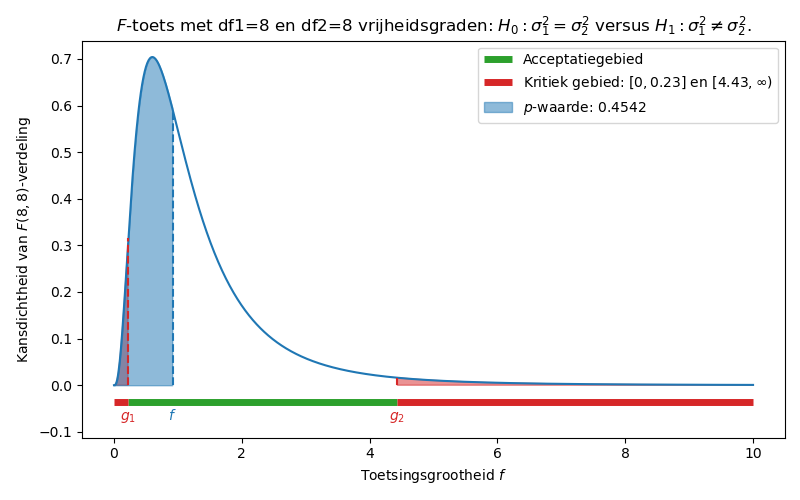
\includegraphics{oefenopgave1_Ftoets.png}
                }
            \end{center}
        }

        \item Bepaal met behulp van een onafhankelijke $t$-toets of de gemiddelde hartslag in stresssituaties bij mannelijke militairen significant hoger ligt dan bij vrouwelijke militairen.
            Baseer je conclusie op het kritieke gebied.
            Kies opnieuw voor het significantieniveau $\alpha = 0,05$.
        \answer{
            We toetsen of de gemiddelde hartslag $\mu_B$ voor mannelijke militairen significant hoger is dan de gemiddelde hartslag $\mu_A$ voor vrouwelijke militairen.
            De hypotheses kunnen we daarom als volgt defini\"eren:
            \begin{align*}
                H_0: \quad \mu_A \ge \mu_B \text{ (niet significant hoger) } \\
                H_1: \quad \mu_A < \mu_B \text{ (wel significant hoger) }
            \end{align*}

            Verder is gegeven dat we mogen werken met een significantieniveau $\alpha=0,05$, en data is al verzameld voor beide populaties.

            Op basis van ons antwoord bij vraag (b) mogen we aannemen dat $\sigma = \sigma_A = \sigma_B$.
            Dat betekent dat we met de pooled variance mogen werken als schatting voor de gemeenschappelijke onbekende $\sigma$.
            
            \begin{align*}
                s_P^2 = \frac{(n-1)\cdot s_A^2 + (m-1) \cdot s_B^2}{n-1+m-1} = \frac{8 \cdot 51,75 + 8 \cdot 56,2778}{16} \approx 54,0139.
            \end{align*}
            
            De toetsingsgrootheid van de bijbehorende $t$-toets is (onder de nulhypothese $\mu_A = \mu_B$) gelijk aan
            \begin{align*}
                t &= \frac{(\overline{x_A}-\overline{x_B}) - (\mu_A - \mu_B)}{\sqrt{\frac{s_P^2}{n} + \frac{s_P^2}{m}}} \\
                  &= \frac{(109,6667 - 119,5556) - 0}{\sqrt{\frac{54,0139}{9} + \frac{54,0139}{9}}} \\
                  &\approx -2,8543, 
            \end{align*}

            en komt uit een $t$-verdeling met $\text{df}=n+m-2=16$ vrijheidsgraden.
            Omdat we linkszijdig toetsen, is het kritieke gebied van de vorm $(-\infty; g]$.
            Deze kritieke grens kunnen we met de $t$-verdeling bepalen, namelijk
            \[
                g = \invt(\text{opp} = \alpha; \text{df}=n+m-2) = \invt(\text{opp}=0,05; \text{df}=16) \approx -1,7459
            \]
            
            De toetsingsgrootheid $t$ ligt dus in het kritieke gebied, dus $H_0$ moet worden verworpen.
            Er is op basis van deze steekproeven voldoende reden om aan te nemen dat de gemiddelde hartslag van mannelijke militairen in stresssituaties significant hoger ligt dan bij vrouwelijke militairen.
            \begin{center}
                \resizebox{0.9\textwidth}{!}{
                    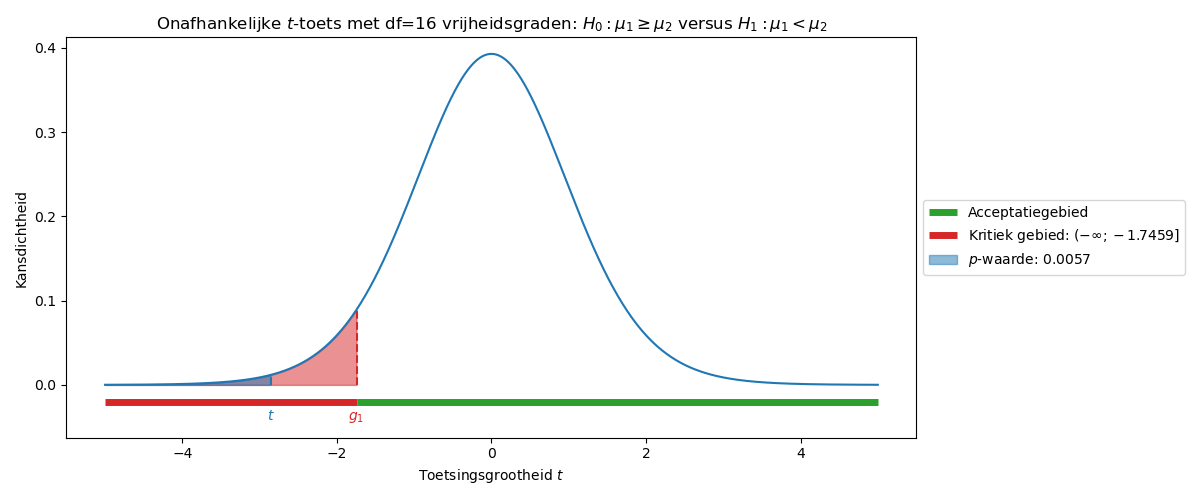
\includegraphics{oefenopgave1_ttoets.png}
                }
            \end{center}
        }    
    
    \end{enumerate}
\question{2}{
    Defensie test de bescherming van een nieuw type scherfvest onder verschillende soorten ballistische dreiging.
    Het onderzoek vindt plaats op het militaire testterrein van de Defensie Materieel Organisatie (DMO).
    Tijdens de test worden twee munitietypen gebruikt: fragmentatiegranaten (groep $A$) en scherpschutterspatronen (groep $B$). 
    In beide gevallen wordt gebruik gemaakt van identieke scherfvesten die zijn bevestigd op testdummies.

    Per vest wordt gemeten hoe diep de kogel- of schervenimpact doordringt in de testdummy, uitgedrukt in millimeters.
    De test wordt uitgevoerd onder gecontroleerde omstandigheden (temperatuur, vocht, afstand en inslaghoek zijn constant).
    Van beide munitietypen worden acht schoten gelost op afzonderlijke vesten, waarna de penetratiediepte wordt gemeten.

    Het hoofd van de testafdeling wil weten of de scherpschutterspatronen significant dieper penetreren dan de fragmentatiegranaten.
    Bij de fragmentatiegranaten werd op basis van een steekproef van 14 metingen een gemiddelde $\overline{x_A} = 9,85$ en variantie $s_A^2 = 0,06$ gemeten.
    Bij de scherpschutterspatronen werd op basis van een steekproef van 17 metingen een gemiddelde $\overline{x_B} = 10,52$ en variantie $s_B^2 = 0,84$ gemeten.

    Voor beide populaties wordt aangenomen dat de gemiddelde hartslag normaal verdeeld is met onbekende verwachtingswaardes $\mu_A$ en $\mu_B$, en standaardafwijkingen $\sigma_A$ en $\sigma_B$.
}
    \begin{enumerate}[label=(\alph*)]
        \item Bepaal met behulp van een $F$-toets of de varianties in de penetratiediepte gelijk zijn voor fragmentatiegranaten en scherpschutterspatronen.
            Gebruik het kritieke gebied in je conclusie. 
            Kies voor het significantieniveau $\alpha = 0,03$.
        \answer{
            In de vraag staat dat we aan mogen nemen dat $X_A \sim N(\mu_A=?; \sigma_A=?)$ en $X_B \sim N(\mu_B=?; \sigma_A=?)$.

            We toetsen op gelijke varianties, oftewel de nulhypothese $H_0$ en de alternatieve hypothese $H_1$ worden als volgt gedefinieerd:
            \begin{align*}
                H_0: \quad \sigma_A^2 = \sigma_B^2 \\
                H_1: \quad \sigma_A^2 \neq \sigma_B^2
            \end{align*}

            Verder is gegeven dat we mogen werken met een significantieniveau $\alpha=0,03$, en data is al verzameld voor beide populaties.
            De toetsingsgrootheid voor een $F$-toets is gelijk aan
            \[
                F = \frac{S_A^2}{S_B^2}, 
            \]
            en volgt een $F(n-1, m-1)$-verdeling, oftewel een $F(13, 16)$-verdeling.

            De geobserveerde toetsingsgrootheid is gelijk aan
            \[
                f = \frac{s_A^2}{s_B^2} = \frac{0,06}{0,84} \approx 0,0714.
            \]
            
            Omdat we tweezijdig toetsen, is het kritieke gebied van de vorm $(-\infty; g_1]$ en $[g_2; \infty)$, waarbij de grenzen $g_1$ en $g_2$ bepaald kunnen worden met de $F(5,9)$-verdeling.
            \begin{align*}
                &\fcdf(\text{lower}=0; \text{upper}=g_1; \text{df1}=13; \text{df2}=16)=\alpha/2=0,015 \rightarrow g_1 \approx 0,2912\\
                &\fcdf(\text{lower}=g_2; \text{upper}=10^{99}; \text{df1}=13; \text{df2}=16)=\alpha/2=0,015 \rightarrow g_2 \approx 3,2041
            \end{align*}
            De berekende $f = 0,0714$ ligt dus in het kritieke gebied, dus we verwerpen de nulhypothese $H_0$.
            Er is op basis van deze steekproeven voldoende bewijs om de aanname van gelijke varianties te verwerpen.
            We mogen dus niet uitgaan van gelijke varianties.

            \begin{center}
                \resizebox{0.9\textwidth}{!}{
                    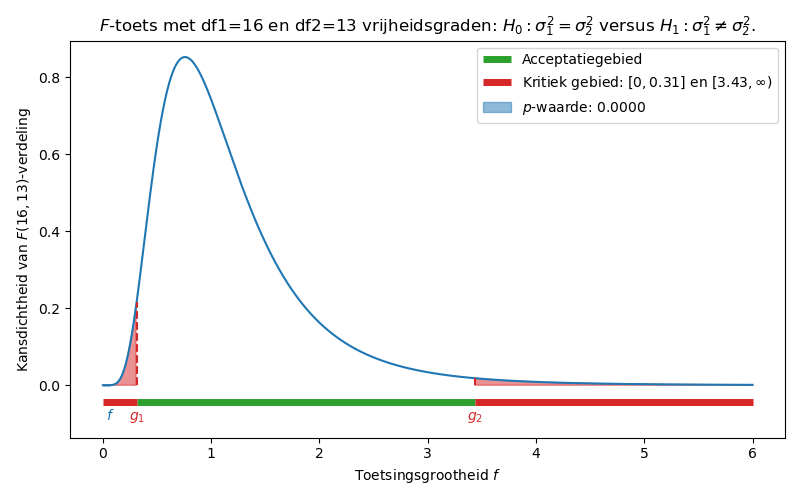
\includegraphics{oefenopgave2_Ftoets.png}
                }
            \end{center}
        }

        \item Bepaal met behulp van een onafhankelijke $t$-toets of scherpschutterspatronen gemiddeld significant dieper in een scherfvest doordringen dan fragmentatiegranaten.
            Formuleer een conclusie op basis van de $p$-waarde.
            Kies opnieuw voor het significantieniveau $\alpha = 0,03$.
        \answer{
            We toetsen of de gemiddelde penetratiediepte $\mu_B$ voor scherpschutterspatronen significant hoger is dan de gemiddelde penetratiediepte $\mu_A$ voor fragmentatiegranaten.
            De hypotheses kunnen we daarom als volgt defini\"eren:
            \begin{align*}
                H_0: \quad \mu_A \ge \mu_B \text{ (niet significant hoger) } \\
                H_1: \quad \mu_A < \mu_B \text{ (wel significant hoger) }
            \end{align*}

            Verder is gegeven dat we mogen werken met een significantieniveau $\alpha=0,03$, en data is al verzameld voor beide populaties.

            Op basis van ons antwoord bij vraag (b) moeten we aannemen dat de standaardafwijkingen $\sigma_A$ en $\sigma_B$ verschillende waardes hebben.
            Dat betekent dat we de onbekende $\sigma_A$ en $\sigma_B$ moeten schatten met respectievelijk $s_A$ en $s_B$:
                       
            De toetsingsgrootheid van de bijbehorende $t$-toets is (onder de nulhypothese $\mu_A = \mu_B$) gelijk aan
            \begin{align*}
                t &= \frac{(\overline{x_A}-\overline{x_B}) - (\mu_A - \mu_B)}{\sqrt{\frac{s_A^2}{n} + \frac{s_B^2}{m}}} \\
                  &= \frac{(9,85 - 10,52) - 0}{\sqrt{\frac{0,06}{14} + \frac{0,84}{17}}} \\
                  &\approx -2,8913, 
            \end{align*}

            en komt uit een $t$-verdeling met $\text{df}=\min(n-1, m-1) = \min(13, 16) = 13$ vrijheidsgraden.
            Omdat we linkszijdig toetsen, is de $p$-waarde gelijk aan de linkeroverschrijdingskans van de waarde $t \approx -2,8913$, oftewel
            \begin{align*}
                p = P(T \le t) = \text{tcdf}(\text{lower}=-10^{99}; \text{upper}=-2,8913; \text{df}=13) \approx 0,0063.
            \end{align*}
            
            Omdat de $p$-waarde kleiner is dan het significantieniveau $\alpha = 0,03$, moet de nulhypothese $H_0$ worden verworpen.
            Er is op basis van deze steekproeven voldoende reden om aan te nemen dat scherpschutterspatronen significant dieper doordringen dan fragmentatiegranaten.
            \begin{center}
                \resizebox{0.9\textwidth}{!}{
                    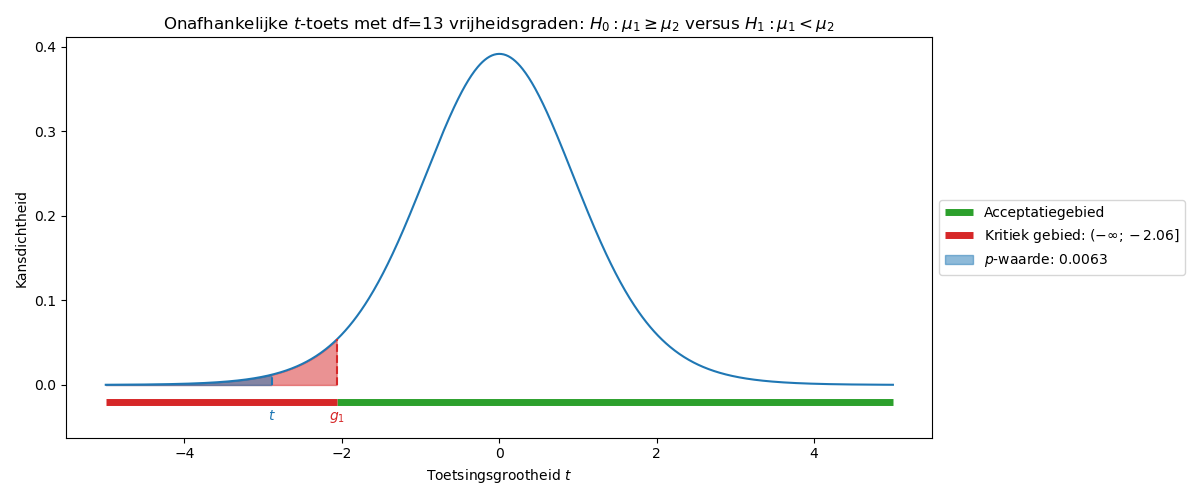
\includegraphics{oefenopgave2_ttoets.png}
                }
            \end{center}
        }    
    
    \end{enumerate}
\question{3}{
    Het Korps Mariniers wil onderzoeken of het klimaat waarin mariniers gestationeerd zijn invloed heeft op hun fysieke conditie.
    Hiervoor wordt de conditie voor twee groepen mariniers gemeten via het maximale zuurstofopnamevermogen ($\text{VO}_2\text{max}$, in ml/kg/min).
    De eerste groep is gestationeerd in het noorden van Noorwegen (koud klimaat, populatie $A$) en de tweede groep in Cura\c{c}ao (warm klimaat, populatie $B$).

    \begin{center}
        \begin{tabular}{c|ccccccccc}
            \toprule
                \textbf{$\text{VO}_2\text{max}$ mariniers in koud klimaat} & $62$ & $60$ & $65$ & $64$ & $61$ & $63$ & $66$ & $64$ \\
                \textbf{$\text{VO}_2\text{max}$ mariniers in warm klimaat} & $58$ & $59$ & $57$ & $60$ & $56$ & $58$ & $59$ & $57$ \\
            \bottomrule
        \end{tabular}
    \end{center}
}
    \begin{enumerate}[label=(\alph*)]
        \item Bereken de steekproefgemiddeldes $\overline{x_A}$ en $\overline{x_B}$, en de steekproefvarianties $s_A^2$ en $s_B^2$.
        \answer{
            {\bfseries Populatie $A$: mariniers in koud klimaat.}
            
            We berekenen het steekproefgemiddelde $\overline{x_A}$ als volgt:
            \begin{align*}
                \overline{x_A} = \frac{x_1+x_2+\ldots+x_n}{n} = \frac{ 62 + 60 + \ldots + 64 }{ 8 } = 63,125
            \end{align*}
        

            We berekenen de steekproefvariantie $s_A^2$ als volgt:
            \begin{align*}
                s_A^2   &= \frac{ (x_1 - \overline{x_A})^2 + (x_2 - \overline{x_A})^2 + \ldots + (x_n - \overline{x_A})^2 }{ n - 1 } \\
                        &= \frac{ (62 - 63,125)^2 + (60 - 63,125)^2 + \ldots + (64 - 63,125)^2 }{ 8 - 1 } \\
                        &\approx 4,125.
            \end{align*}
       
            {\bfseries Populatie $B$: mariniers in warm klimaat.}

            We berekenen het steekproefgemiddelde $\overline{x_B}$ als volgt:
            \begin{align*}
                \overline{x_B} = \frac{x_1+x_2+\ldots+x_n}{n} = \frac{ 58 + 59 + \ldots + 57 }{ 8 } = 58
            \end{align*}
        

            We berekenen de steekproefvariantie $s_B^2$ als volgt:
            \begin{align*}
                s_B^2   &= \frac{ (y_1 - \overline{x_B})^2 + (y_2 - \overline{x_B})^2 + \ldots + (y_n - \overline{x_B})^2 }{ m - 1 } \\
                        &= \frac{ (58 - 58)^2 + (59 - 58)^2 + \ldots + (57 - 58)^2 }{ 8 - 1 }\\
                        &\approx 1,7143.
            \end{align*}       
        }

        \item Bepaal met behulp van een $F$-toets of de varianties in $\text{VO}_2\text{max}$ gelijk zijn voor beide groepen mariniers.
            Gebruik het kritieke gebied in je conclusie. 
            Kies voor het significantieniveau $\alpha = 0,05$.
        \answer{
            In de vraag staat dat we aan mogen nemen dat $X_A \sim N(\mu_A=?; \sigma_A=?)$ en $X_B \sim N(\mu_B=?; \sigma_A=?)$.

            We toetsen op gelijke varianties, oftewel de nulhypothese $H_0$ en de alternatieve hypothese $H_1$ worden als volgt gedefinieerd:
            \begin{align*}
                H_0: \quad \sigma_A^2 = \sigma_B^2 \\
                H_1: \quad \sigma_A^2 \neq \sigma_B^2
            \end{align*}

            Verder is gegeven dat we mogen werken met een significantieniveau $\alpha=0,05$, en data is al verzameld voor beide populaties.
            De toetsingsgrootheid voor een $F$-toets is gelijk aan
            \[
                F = \frac{S_A^2}{S_B^2}, 
            \]
            en volgt een $F(n-1, m-1)$-verdeling, oftewel een $F(13, 16)$-verdeling.

            De geobserveerde toetsingsgrootheid is gelijk aan
            \[
                f = \frac{s_A^2}{s_B^2} = \frac{4,125}{1,7143} \approx 2,4062.
            \]
            
            Omdat we tweezijdig toetsen, is het kritieke gebied van de vorm $(-\infty; g_1]$ en $[g_2; \infty)$, waarbij de grenzen $g_1$ en $g_2$ bepaald kunnen worden met de $F(5,9)$-verdeling.
            \begin{align*}
                &\fcdf(\text{lower}=0; \text{upper}=g_1; \text{df1}=7; \text{df2}=7)=\alpha/2=0,025 \rightarrow g_1 \approx 0,2002\\
                &\fcdf(\text{lower}=g_2; \text{upper}=10^{99}; \text{df1}=7; \text{df2}=7)=\alpha/2=0,025 \rightarrow g_2 \approx 4,9949
            \end{align*}
            De berekende $f = 2,4062$ ligt dus niet in het kritieke gebied, dus we mogen de nulhypothese $H_0$ accepteren.
            Er is op basis van deze steekproeven onvoldoende bewijs om de aanname van gelijke varianties te verwerpen.
            We mogen dus uitgaan van gelijke varianties en de gemeenschappelijke $\sigma = \sigma_A = \sigma_B$ schatten aan de hand van de ``pooled variance''.

            \begin{center}
                \resizebox{0.9\textwidth}{!}{
                    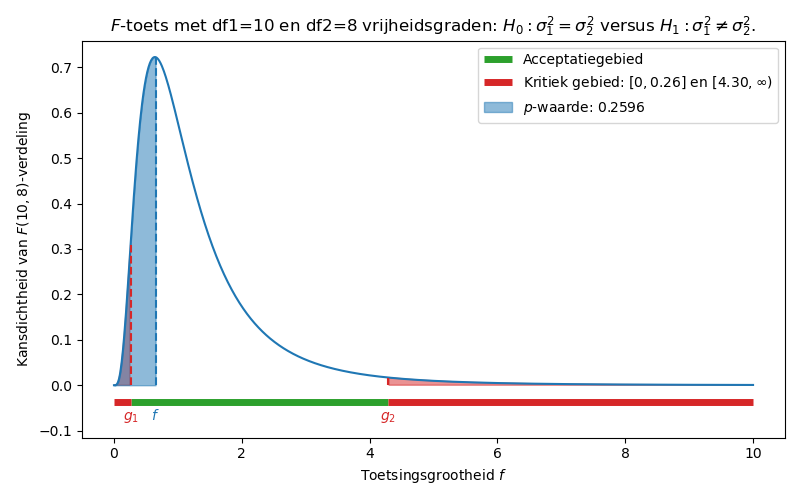
\includegraphics{oefenopgave3_Ftoets.png}
                }
            \end{center}
        }

        \item Bepaal met behulp van een onafhankelijke $t$-toets of de gemiddelde $\text{VO}_2\text{max}$-waardes significant van elkaar afwijken
        voor beide groepen mariniers.
            Formuleer een conclusie op basis van de $p$-waarde.
            Kies opnieuw voor het significantieniveau $\alpha = 0,05$.
        \answer{
            We toetsen of de gemiddelde $\text{VO}_2\text{max}$-waardes $\mu_B$ voor de populaties mariniers in respectievelijk koude en warme klimaten significant van elkaar afwijken.
            De hypotheses kunnen we daarom als volgt defini\"eren:
            \begin{align*}
                H_0: \quad \mu_A = \mu_B \text{ (geen significant afwijking) } \\
                H_1: \quad \mu_A \neq \mu_B \text{ (wel een significante afwijking) }
            \end{align*}

            Verder is gegeven dat we mogen werken met een significantieniveau $\alpha=0,05$, en data is al verzameld voor beide populaties.

            Op basis van ons antwoord bij vraag (b) mogen we aannemen dat $\sigma = \sigma_A = \sigma_B$.
            Dat betekent dat we met de pooled variance mogen werken als schatting voor de gemeenschappelijke onbekende $\sigma$.
            
            \begin{align*}
                s_P^2 = \frac{(n-1)\cdot s_A^2 + (m-1) \cdot s_B^2}{n-1+m-1} = \frac{7 \cdot 4,125 + 7 \cdot 1,7143}{14} \approx 2,9196.
            \end{align*}
            
            De toetsingsgrootheid van de bijbehorende $t$-toets is (onder de nulhypothese $\mu_A = \mu_B$) gelijk aan
            \begin{align*}
                t &= \frac{(\overline{x_A}-\overline{x_B}) - (\mu_A - \mu_B)}{\sqrt{\frac{s_P^2}{n} + \frac{s_P^2}{m}}} \\
                  &= \frac{(63,125 - 58) - 0}{\sqrt{\frac{2,9196}{9} + \frac{2,9196}{9}}} \\
                  &\approx 5,9987. 
            \end{align*}

            en komt uit een $t$-verdeling met $\text{df}=n+m-2 = 8 + 8 - 2 = 14$ vrijheidsgraden.
            Omdat we tweezijdig toetsen, is de $p$-waarde gelijk aan de rechteroverschrijdingskans van de waarde $t \approx 5,9987$ (deze is kleiner dan de linkeroverschrijdingskans omdat de $t$-verdeling symmetrisch rond $0$ is), oftewel
            \begin{align*}
                p = P(T \ge t) = \text{tcdf}(\text{lower}=5,9987; \text{upper}=10^{99}; \text{df}=13) \approx 1,6310 \cdot 10^{-5}.
            \end{align*}
            
            Omdat de $p$-waarde (veel) kleiner is dan het significantieniveau $\alpha = 0,05$, moet de nulhypothese $H_0$ worden verworpen.
            Er is op basis van deze steekproeven voldoende reden om aan te nemen dat de gemiddelde $\text{VO}_2\text{max}$-waardes van mariniers die in respectievelijk koude en warme klimaten gestationeerd zijn, significant van elkaar afwijken.
            \begin{center}
                \resizebox{0.9\textwidth}{!}{
                    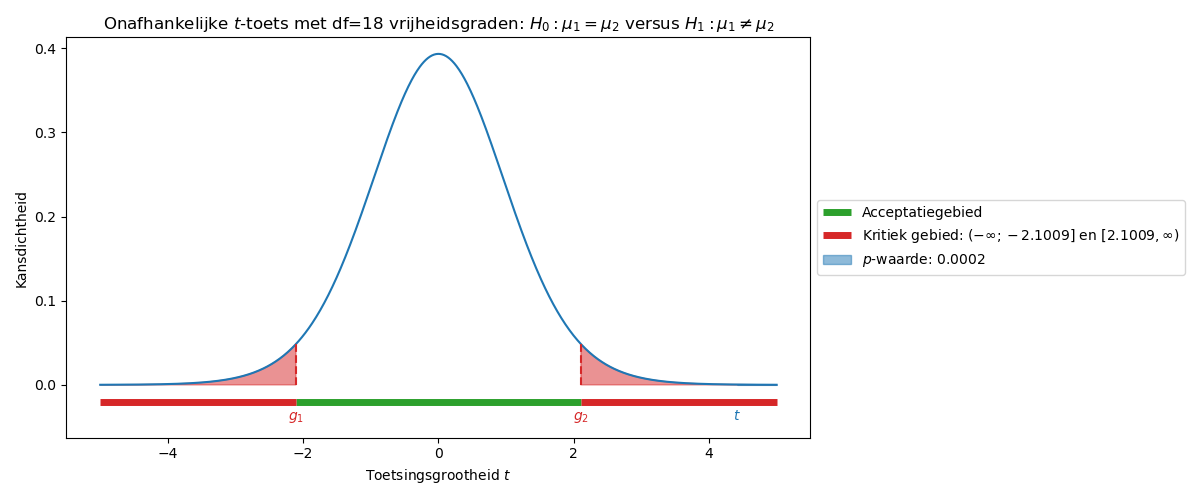
\includegraphics{oefenopgave3_ttoets.png}
                }
            \end{center}

            {\itshape Side note: bij dit soort vragen is het interessant om te kijken wat de toetsuitslag ons nu eigenlijk zegt en hoe dat te verklaren is.
            De toetsuitslag geeft aan dat er een significante afwijking is, maar niet de richting.
            Uit de data is echter op te maken dat de $\text{VO}_2\text{max}$-waardes vrijwel consistent hoger liggen voor de mariniers in het koude klimaat.
            Wellicht heeft dit te maken met het feit dat in koude klimaten minder zuurstof in de lucht zit.
            Het lichaam moet dan zelf harder werken en meer rode bloedlichaampjes produceren om genoeg zuurstof binnen te krijgen, waardoor de zuurstofopname verbeterd wordt.}
        }    
    
    \end{enumerate}


\end{document}